\documentclass[11pt]{scrartcl}
\usepackage[utf8]{inputenc} % Kodierung der Textdatei mit Sonderzeichen
\usepackage[ngerman]{babel} % Sprache fuer Inhaltsverzeichnis etc.
\usepackage{amssymb} % Mathematische Symbole
\usepackage{amsmath} % Mehr mathematische Konstrukte
\usepackage{graphicx} % Um Bilder einbinden zu koennen
\usepackage{float} % fuer \begin{figure}[H]
\usepackage{icomma} % laesst das Komma als Dezimaltrennzeichen interpretieren
\usepackage{fix-cm} % für die große Titelschrift
\usepackage[pdftex]{hyperref} % Hyperlinks im Dokument
\hypersetup{colorlinks=true, linkcolor=black, citecolor=black, filecolor=black, urlcolor=black, pdftitle={LED-Spektrometer - Projektpraktikum 09/10 Gruppe 5}}


\newcommand{\unit}[1]{\ensuremath{\,\mathrm{#1}}} % Einheiten schreiben sich immer aufrecht!
\newcommand{\degr}{\ensuremath{^\circ}}
\newcommand{\cel}{\ensuremath{\degr\mathrm{C}}}
\newcommand{\dif}{\ensuremath{\mathrm{d}}}
\newcommand{\pdif}[2]{\ensuremath{\frac{\partial#1}{\partial#2}}}
\newcommand{\ee}[1]{\ensuremath{\cdot 10^{#1}}}
\newcommand{\hypref}[2]{\hyperref[#2]{{#1}~\ref{#2}}}

\setlength{\parindent}{1em}
\setlength{\parskip}{0.5\baselineskip}


\title{Direkte Messung der Erdrotation - Gruppe 5 WS 09/10, Projektpraktikum der Uni Erlangen}
\date{07.12.2009 -- 15.01.2010}
\author{Michele Collodo, Andreas Glossner, Karl-Christoph G\"odel, Bastian Hacker, Maria Obst, Alexander Wagner, David Winnekens}



\begin{document}
\sloppy % laesst Latex nicht ueber den Rand rausschreiben
\thispagestyle{empty}
\large{Projektpraktikum WS 09/10}
\hfill
\raisebox{-1.4cm}{
\includegraphics[width=5cm]{images/fau.pdf}}
\\[8\baselineskip]
\begin{center}
{\fontsize{36}{54}\textbf{Direkte Messung der Erdrotation}}
\\[2\baselineskip]
{\Large 07.12.2009 -- 15.01.2010}
\\[7\baselineskip]
{\huge\textbf{PPG 5}}
\\[0.5\baselineskip]
{\large\textbf{
Michele Collodo,
Andreas Glossner,\\
Karl-Christoph G\"odel,
Bastian Hacker,\\
Maria Obst,
Alexander Wagner,
David Winnekens}\\
Tutor: Xiaoyue Jin}
\vfill



\small{\url{http://pp.physik.uni-erlangen.de/groups/ws0910/ppg5/ppg5\_start.html}}
\end{center}
\newpage



\tableofcontents
\vfill



\begin{abstract}
Bla Abstract Bla
\end{abstract}
\newpage

\section{Einleitung} %Michele
Messung der Erdrotation - eines der \"altesten Experimente der Physik

\section{Grundprinzip - Tr\"agheitsmoment}

\begin{figure}[ht]
\begin{center}
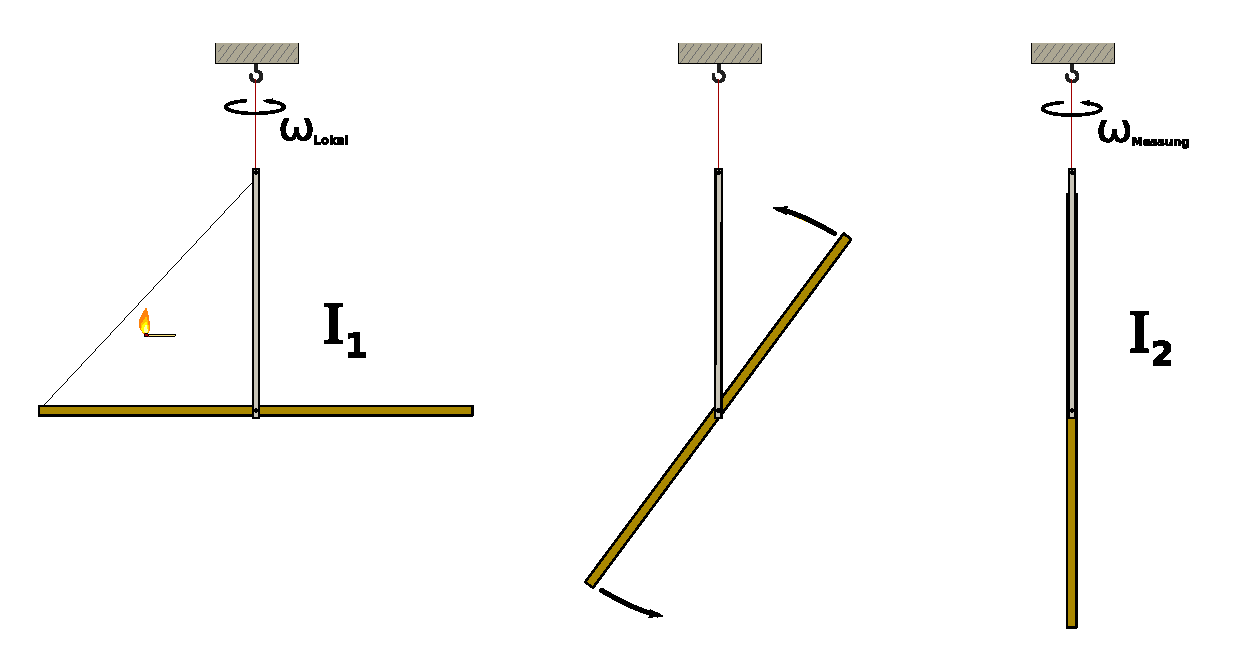
\includegraphics[width=0.8\textwidth]{images/prinzip.pdf}
\end{center}
\vspace{-1.5\baselineskip}
\caption{Schema des Bewegungsablaufs}
\label{prinzip}
\end{figure}

\begin{figure}[ht]
\begin{center}
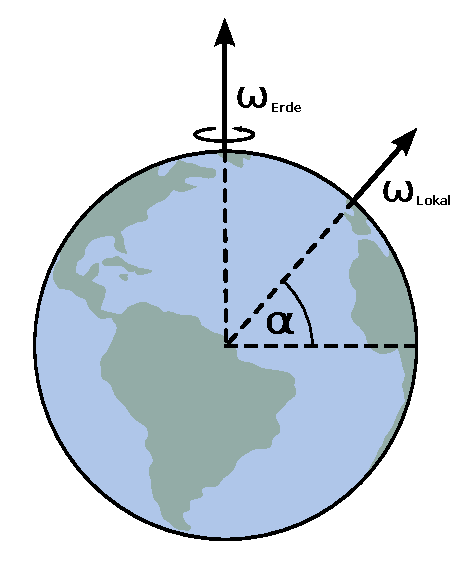
\includegraphics[width=0.2\textwidth]{images/welt.pdf}
\end{center}
\vspace{-1.5\baselineskip}
\caption{Position auf der Welt}
\label{Welt}
\end{figure}


\section{Bau des Drehstabs} %Maria (solltest du nicht zu allem was wissen, sag bescheid)
\subsection{Material}
Magnetismus, Verwindung usw.
\subsection{Aufh\"angung}
Stabilisierung der Drehbewegung
\subsection{Klappmechanismus}
Zugmechanismus, Einrasten

\begin{figure}[ht]
\begin{center}
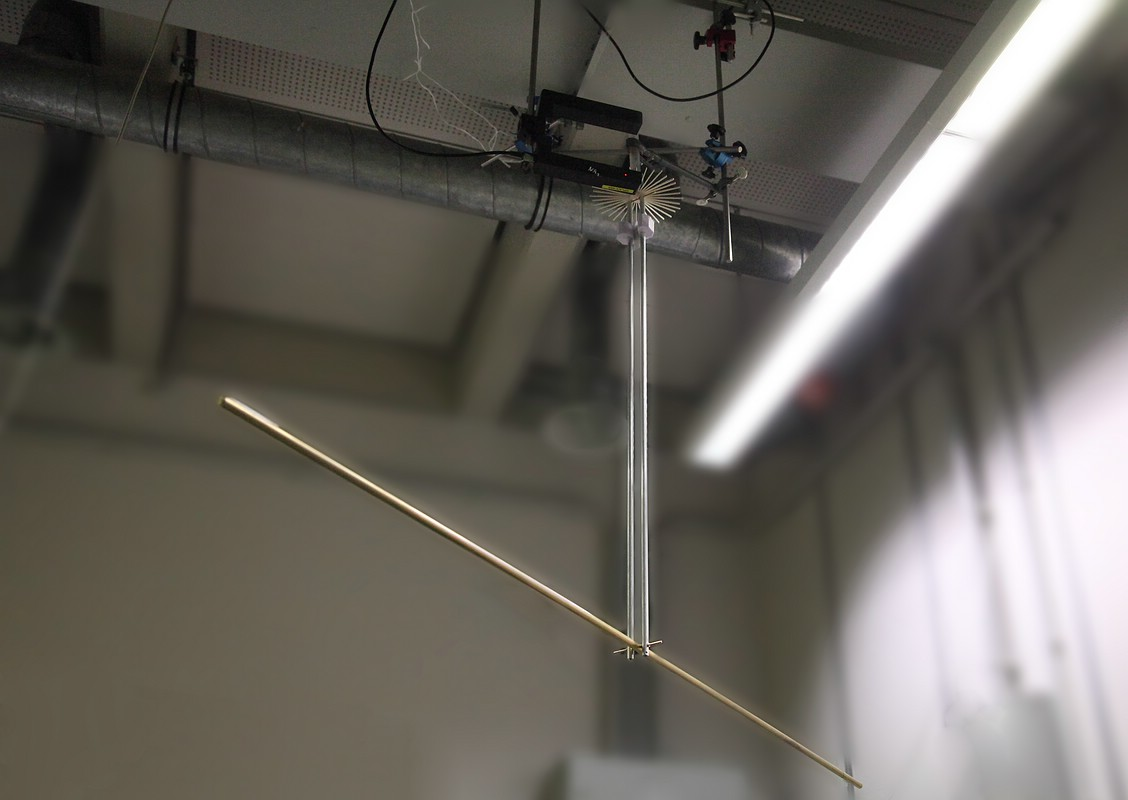
\includegraphics[width=0.8\textwidth]{images/stab-fertig.jpg}
\end{center}
\vspace{-1.5\baselineskip}
\caption{Der ausgelenkte Stab}
\label{stab-fertig}
\end{figure}

\section{Messungen}
\subsection{Berechnungen im Vorraus} %Andi
Tr\"agheitsmoment Rechnungen von Andi

\subsection{Cassymessungen} %Axi
Zur Aufzeichnung der Drehung des Stabes kam zun\"achst das CASSY Lab System zum Einsatz. Auf der H\"ohe der Spitze des Stabes wurde eine Lichtschranke durch Stativstangen an der Deckenkonstruktion verschraubt, welche die Durchg\"ange des Stabes z\"ahlte. Die Ausl\"osung der Lichtschranke sollte durch einen leichten Querstab aus Balsaholz erfolgen. Es stellte sich jedoch heraus, dass dabei nur unzureichende Genauigkeiten bei der Ermittlung der Drehgeschwindikeit erzielt werden konnten, da die Lichtschranke bei dieser Methode nur zweimal pro ganzer Umdrehung ausgel\"ost wird. Deshalb wurde an der Spitze des Stabes ein \glqq Speichenrad\grqq installiert. Die einzelnen Speichen hatten dabei einen Abstand von jeweils $10^\circ$. Pro Umdrehung wurde die Schranke also 36 Mal ausgel\"ost. Die L\"ange der Speichen wurde so kurz wie m\"oglich gehalten um das Tr\"agheitsmoment des Stabes nicht unn\"otig zu beeinflussen.

\begin{figure}[h]
\begin{center}
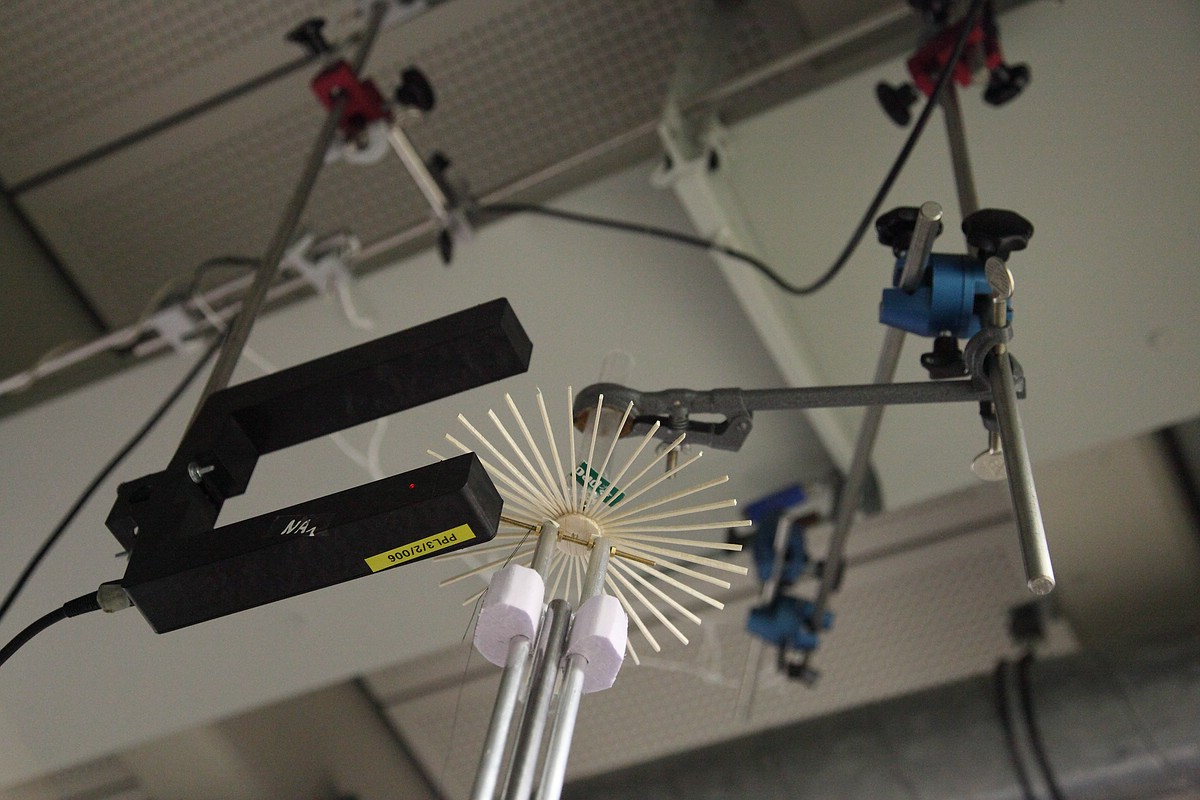
\includegraphics[width=0.8\textwidth]{images/lichtschranke.jpg}
\end{center}
\vspace{-1.5\baselineskip}
\caption{Das Speichenrad beim Durchgang durch die Lichtschranke}
\label{lichtschranke}
\end{figure}

\subsection{Videomessungen} %Karl
Da die Schwingung der Vorrichtung die Cassymessung fast unbrauchbar machte, wurden weitere Wege gesucht, die bisherigen Versuche dennoch auswertbar zu machen. Als Grundlage sollten hier Videoaufnahmen dienen, die es ermöglichten, die Drehung unmittelbar nach dem Einklappen des Stabes zu beschreiben, bevor die störende Schwingung den Effekt zu stark überlagert. Die zur verfügung stehenden Mitschnitte wurden ursprünglich nur zu Dokumentationszwecken aufgezeichnet. Dies hatte den Nachteil, dass die Videodateien vor der Auswertung noch stark bearbeitet werden mussten, um Messdaten ablesen zu können. Das Hauptproblem lag in der verzerrten Perspektive des Videos, das von schräg unten aufgenommen wurde (siehe Abbildung ?). Zur Auswertung wurde mit Hilfe der freien Bildbearbeitungssoftware GIMP wie folgt vorgegangen: Zuerst wurde das Video in seine Einzelbilder zerlegt. Anhand dieser Bilder, im Speziellen der sich drehenden, oberen Verbindungsquerstange, wurde durch fitten einer Ellipse die perspektivische Verzerrung ermittelt. Für das Halbachsenverhältnis dieser Ellipse ergab sich folgender Wert:
\[\frac{a_{groß}}{a_{klein}}=3,21\]
Nun wurden die Einzellbilder senkrecht ausgerichtet, also um den Winkel $\alpha$ gedreht (siehe Abbildung ? - A) und schließlich um den ermittelten Faktor $3,21$ gestreckt (siehe Abbildung ? - B).
\begin{figure}[h]
\begin{center}
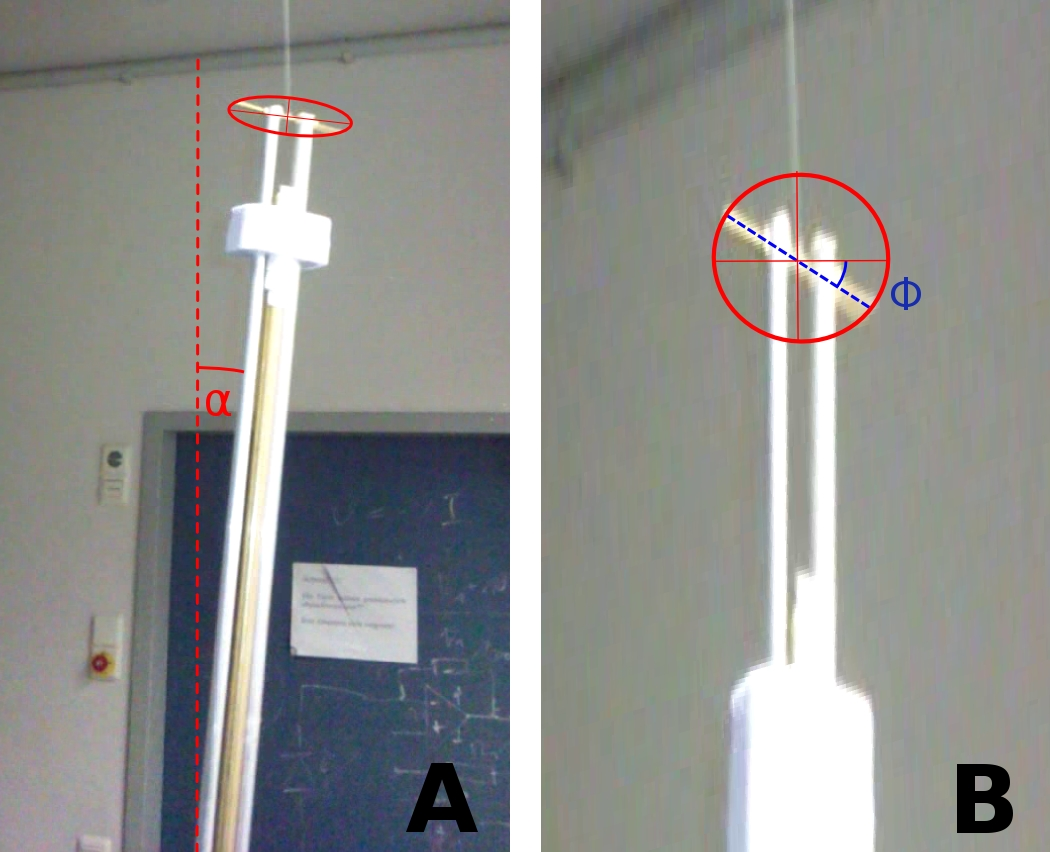
\includegraphics[width=0.8\textwidth]{images/auswert.jpg}
\end{center}
\vspace{-1.5\baselineskip}
\caption{Bearbeitung der Videoeinzelbilder}
\label{Videobearbeitung}
\end{figure}
Aus diesen Bilddaten konnten nun der Drehwinkel $\phi$ abgelesen werden. Der Fehler dieser Messung lag vor allem in der unterschiedlichen Qualität der Einzelbilder und wurde durch mehrmaliges Messen pro Bild ermittelt.
Da die schon anfänglich erwähnte Schwankung leider sehr schnell nach dem Einklappvorgang ins Gewicht fiel, konnten nur einige wenige Messpunkte zur Ermittlung der Winkelgeschwindigkeit herangezogen werden.
\begin{figure}[h]
\begin{center}
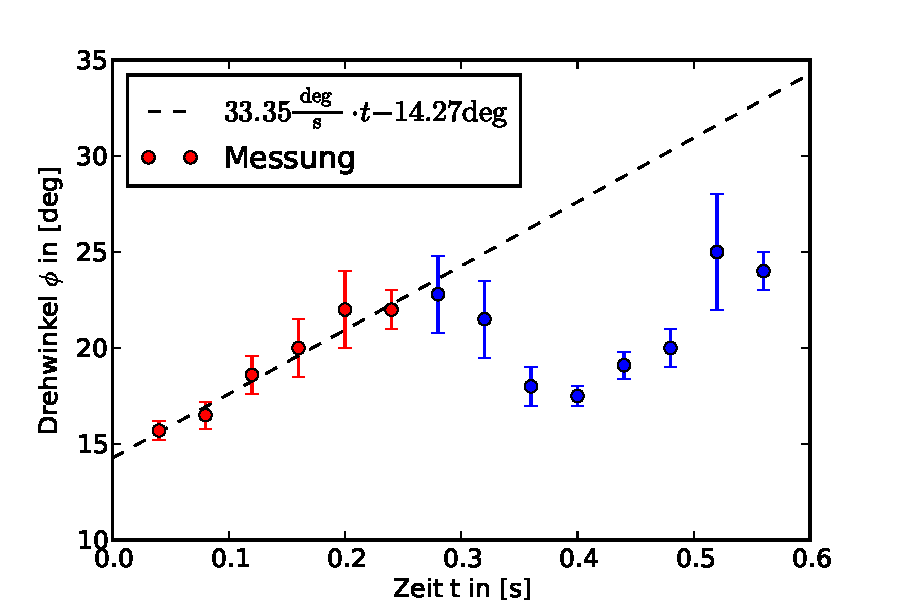
\includegraphics[width=0.8\textwidth]{images/messung_Video.pdf}
\end{center}
\vspace{-1.5\baselineskip}
\caption{Messergebnisse der Video-Messung}
\label{messung_Video}
\end{figure}
Der zeitliche Abstand der Videoeinzelbilder wurde mit Hilfe einer Stoppuhr zu $\Delta t = 0,04\unit{s}$ gemessen.
Durch einen Geradenfit der ersten sechs Messpunkte wurde die Winkelgeschwindigkeit ermittelt. Es gilt:
\[ \omega_{Messung} = 33,35 \frac{\unit{deg}}{\unit{s}} = 0,582 \unit{Hz} \]
Damit ergibt sich mit den bekannten Werten für die Trägheitsmomente folgende Winkelgeschwindigkeit der Erdrotation:
\[ \omega_{Erde} = \frac{\omega_{lokal}}{\unit{sin}(\alpha)} = ... \]


\section{Verbesserungsvorschläge} %David faden, zwei stäbe, kamera von oben, symmetrischerer aufbau


\section{Fazit} %Basti
Nicht alles funktioniert so, wie erwartet \dots $\rightarrow$ Warum?

\end{document}
